% $Id: theory.tex,v 1.1 1999/07/16 20:32:37 dosuser Exp dosuser $

% commands.tex
% Jeremy Barnes, 1999
% $Id$

\providecommand{\emp}{\mathrm{emp}}
\providecommand{\calF}{\ensuremath{\mathcal{F}}}
\providecommand{\fat}{\ensuremath{\mathrm{fat}}}
\providecommand{\sign}{\ensuremath{\mathrm{sign}}}
\providecommand{\cop}{\ensuremath{\mathrm{co}_p}}
\providecommand{\co}{\ensuremath{\mathrm{co}}}
\providecommand{\bfx}{\ensuremath{\mathbf{x}}}
\providecommand{\bfy}{\ensuremath{\mathbf{y}}}
\providecommand{\bfyh}{\ensuremath{\hat{\mathbf{y}}}}
\providecommand{\calO}{\ensuremath{\mathcal{O}}}
\providecommand{\calI}{\ensuremath{\mathcal{I}}}
\providecommand{\calH}{\ensuremath{\mathcal{H}}}
\providecommand{\calX}{\ensuremath{\mathcal{X}}}
\providecommand{\ip}[2]{\ensuremath{\langle {#1} , {#2} \rangle}}
\providecommand{\lin}{\mathrm{lin}}
\providecommand{\calS}{\ensuremath{\mathcal{S}}}
\providecommand{\VCdim}{\mathrm{VCdim}}
\providecommand{\Fat}[1]{\mathrm{Fat}_{#1}}
\providecommand{\cover}[2]{\mathcal{N}({#1}, {#2})}
\providecommand{\covert}[3]{\mathcal{N}({#1}, {#2}, {#3})}
\providecommand{\MATLAB}{{\tt MATLAB}}
\providecommand{\C}{{\tt C}}
\providecommand{\argmin}{\mathrm{argmin}}

% Theorem-like constructs
\newtheorem{theorem}{Theorem}
\newtheorem{definition}{Definition}

\providecommand{\proof}{\par \par \noindent {\bf Proof:\ }}

\providecommand{\figlinewidth}{1pt}

\newenvironment{linefigure}%
		{\begin{figure} \rule{\textwidth}{\figlinewidth}}%
		{\rule{\textwidth}{\figlinewidth}\end{figure}}


\chapter{Background theory}
\label{chapter:theory}

This chapter contains a brief summary of the main theoretical results
necessary to understand the rest of the report.  Familiarity with the
field of statistical learning theory is assumed.  A general overview
of this field is available in \cite{Cherkassky98}.


\section{Notation}

We begin with definitions and notation.  A classifier is a hypothesis
with a discrete output set.  It is characterised by a
function $f(\cdot) : \mathcal{I} \mapsto \mathcal {O}$.  For the
classifiers in this report, we will use $\calI = [0,1] \times [0,1]$ (two
dimensional) and $\calO = \{-1,1\}$ (binary) for simplicity.
\footnote{Generalisation to other situations is not
usually difficult (see for example \cite{Freund96} and
\cite{Cherkassky98}).}  Samples are notated $\{\bfx, \bfy\}$ where
$\bfx \in \calI$ is the attribute vector and $\bfy \in \calO$ the
class.  A hypothesis $f(\cdot)$ given an attribute vector \bfx\
produces a class $y = f(\bfx)$.

The ``weak'' learning algorithms decision stumps and CART are
described in appendix \ref{chapter:weak learners}.  Weak learning
algorithms are notated $f_i(\cdot)$; $i$ is an
index and each $f_i$ is an element of \calF, which is the set of all
\emph{compatible} instances of a learning algorithm.  A learning
algorithm is compatible with a problem if the domain \calI\ and range
\calO\ match.


\section{Boosting}

AdaBoost is a machine learning algorithm
that combines many ``weak'' hypotheses to generate a hypothesis 
that usually performs significantly better than any of the weak
hypotheses.  Even the simplest of weak algorithms, when
boosted, will usually outperform the best unboosted algorithms.
\footnote{As a result, the focus of recent research effort has shifted from the
development of \emph{learning} algorithms (which are all more
or less equivalent when boosted) to the development of better \emph{boosting}
algorithms.}

These weak hypotheses are combined in a linear combination.
The weight of each weak hypothesis (the
\emph{classifier weight}) depends upon the performance of that
classifier on the training dataset.  Section \ref{sec:classifier
weights} describes these classifier weights in more detail.

Each sample in the training dataset is given a weight (\emph{sample
weight}) which is modified depending upon how ``hard'' that
sample is to classify.  Section \ref{sec:sample weights} describes
these sample weights in more detail.

A more thorough description of boosting is given in appendix
\ref{chapter:boosting details} and \cite{Freund96}.

\subsection{Classifier weights}
\label{sec:classifier weights}

The AdaBoost algorithm combines a number of ``weak'' classifiers
$f_1(\cdot), \ldots, f_n(\cdot)$ in a linear combination to produce a
``stronger'' classifier $F(\cdot) = \sum_{i=1}^{n} b_i f_i(\cdot)$.
The coefficients $b_i$ are subject to the condition that they produce a
convex combination where $\|b\|_1 = \sum_{i=1}^{t} b_i = 1$.

AdaBoost's training process is divided into iterations.  On iteration
$t$, one weak learner $f_t(\cdot)$ is added to the linear
combination ($f_t$ is chosen by the weak learning algorithm).  The
coefficient $b_t$ of $f_t$ is calculated from the 
training error $\epsilon_t$ of $f_t$ as 
%
\begin{equation}
b_t = - \log \frac{\epsilon_t}{1 - \epsilon_t}
\label{eqn:theory:bt}
\end{equation}
%
When $\epsilon_t = 1/2$, the classifier only does as
well as random guessing, and has $b_t = 0$.  As
$\epsilon_t$ approaches zero, $b_t$ increases without bound.  The
effect is that $F$ becomes dominated by those weak hypotheses that
performed well on the training samples
\footnote{Training is halted if $\epsilon_t = 0$ or $\epsilon_t \geq 1/2$.}.  The weights are normalised once training is completed.


\subsection{Sample weights}
\label{sec:sample weights}

Each sample in the training set has a corresponding weight $w_j$ which
is updated to reflect the difficulty of that sample.  On each iteration the
weights of samples which $f_t$ classified incorrectly are increased
(scaled by $\exp \{ -b_t \}$); the whole lot are then normalised.
This function has the following effect on distribution of weights:

\begin{itemize}

\item	Training samples which are misclassified often, or are one of 
	few points to get misclassified, increase their proportion of
	the weight (are identified as ``hard samples'');

\item	Other samples decrease their proportion of the weight, and are
	identified as ``easy'' samples.

\end{itemize}

The overall effect is for those samples near the decision boundary to
increase in weight, and those far from it to decrease.  This forces
the algorithm to concentrate on the hard samples, and is one reason
why it works well on low-noise datasets.  Unfortunately, those samples
corrupted by noise are usually hard also, and concentrating on those
is not desirable.


\section{Boosting as gradient descent}
\label{sec:theory:gradient descent}

Recent work has shown boosting to be an implementation of gradient
descent in an inner product space \cite{Mason99}\footnote{This
discussion follows Mason et al. \cite{Mason99} rather closely with
some changes in notation and omission of details such as stopping
criteria.}.
An inner product space requires both a universal set
$\mathcal{X}$ and an inner product operator \ip{\cdot}{\cdot}.  We
define
%
\begin{equation}
\calX = 
\mathrm{co} (\calF) \doteq
 \bigcup _{n \in \mathbb{N}}
\left\{
 \sum_{i=1}^{n}
  b_i
f_i : f_1, \ldots, f_n \in \calF,
 b_1, \ldots, b_n \in \mathbb{R},
 \sum_{i=1}^{n} | b_i | = 1
\right\} \cup \emptyset
\end{equation}
%
(which is the convex hull of \calF), and
%
\begin{equation}
\ip{F}{G} = \frac{1}{l} \sum_{i=1}^{l} F(\bfx_i)G(\bfx_i) \qquad
F, G \in \calX
\end{equation}
%
We also choose the cost function
%
\begin{equation}
C(F) = \frac{1}{l} \sum_{i=1}^{l} \exp
\left\{ -y_i F(\bfx_i) \right\}
\label{eqn:theory:cost function}
\end{equation}

At iteration $t$ of gradient descent, we wish to choose a function $f_t$ and
a weight $b_t$ such that $C(F + b_t f_t)$ decreases (the choice of
$f_t$ is made indirectly through the choice of the sample weights
$w|_t$).  In other words, we are asking for sample weights $w|_t$ that
choose a \emph{direction} $f_t \in \calF$ such that $C(F + b_t f_t)$
decreases as fast as possible.  This direction is the negative of the
functional derivative of $C$:
%
\begin{equation}
f = -\nabla C(F)(\bfx) = \left. \frac{\partial C(F + \alpha
1_{\bfx})}{\partial \alpha} \right|_{\alpha = 0}
\label{eqn:functional derivative}
\end{equation}
%
where $1_{\bfx}$ is the indicator function of $\bfx$; this is
necessary as we can only evaluate \ref{eqn:functional derivative} at
points where we have a sample.  Since the
optimal $f_t$ will not necessarily be in $\calF$, we choose the
$f \in \calF$ with the greatest inner product $\ip{-\nabla
C(F)}{f}$.

Having chosen our direction, we now choose a step size $b_t$.
AdaBoost uses a line search for the minimum of the cost functional
along this line
%
\begin{equation}
b_t = \arg \min_{b_t} \sum_{i=1}^{l} C(y_i F(\bfx_i) + y_i b_t f_t(\bfx_i)
\end{equation}
%
which (for the cost function (\ref{eqn:theory:cost
function})) has a closed-form solution  (\ref{eqn:theory:bt}).  Thus, the
boosting algorithm implements gradient descent.  The process is
illustrated in figure \ref{fig:gradient descent}.

\begin{figure}
\begin{center}
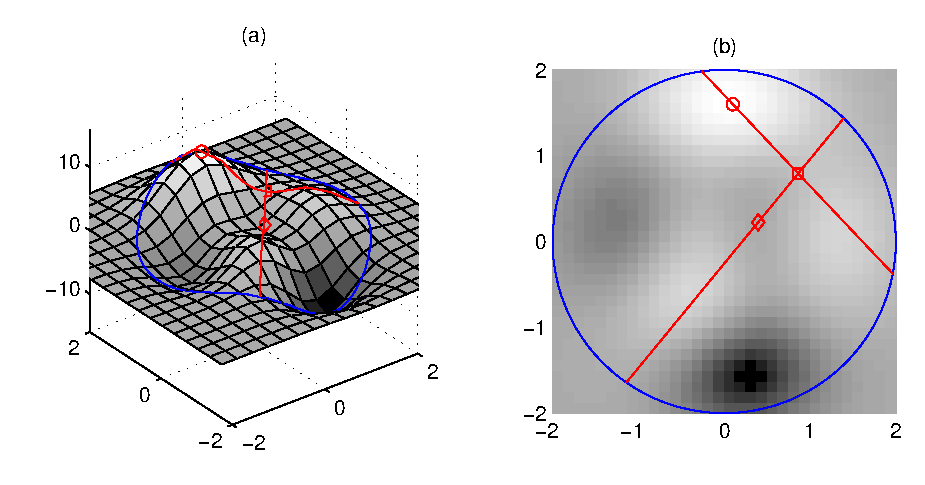
\includegraphics{figures/descent.eps}
\caption{Schematic representation of gradient descent.  Points within the blue
circle are in \calF, the height of the surface the value of
(\ref{eqn:theory:cost function}) at that point.  (a) is a 3D view, (b)
is top view. Red lines show line searches; markers minimums.  Descent
from $\circ$ to $\Box$ to $\Diamond$, where it terminates due to
local minimum.}
\label{fig:gradient descent}
\end{center}
\end{figure}




